%%% Local Variables:
%%% coding: utf-8
%%% mode: latex
%%% TeX-engine: xetex
%%% End:
\documentclass[10pt]{beamer}
% NOTE May need to manually set tex engine in emacs

\usetheme[progressbar=frametitle]{metropolis}
\usepackage{appendixnumberbeamer}

\usepackage{svg}
\usepackage{ulem}
\usepackage{cancel}
\usepackage{wrapfig}
\usepackage{fancyvrb}
\usepackage{hyperref}
\usepackage{cleveref}
\usepackage{stmaryrd}
\usepackage{amsmath}
\usepackage{listings}

\usepackage{pifont}
\newcommand{\cmark}{\ding{51}}
\newcommand{\xmark}{\ding{55}}

\usepackage[dvipsnames]{xcolor}
\definecolor{mLightGreen}{HTML}{14B03D}

\usepackage{booktabs}
\usepackage[scale=2]{ccicons}

\usepackage{graphicx}

\usepackage{pgfplots}
\usepgfplotslibrary{dateplot}

\usepackage{todonotes}
\newif\ifdraft
\drafttrue
\newcommand{\todoin}[1]{\ifdraft{\todo[inline]{TODO:\@ #1}}\fi}

\usepackage{xspace}
\usepackage{mathpartir}
\newcommand{\themename}{\textbf{\textsc{metropolis}}\xspace}

\newcommand{\sem}[1]{\llbracket{#1}\rrbracket}
\newcommand{\cat}[1]{\mathbf{#1}}
\newcommand{\lto}{\multimap}
\newcommand{\tol}{\mathrel{\rotatebox[origin=c]{180}{$\lto$}}}
\newcommand{\String}{\Sigma^{*}}
\newcommand{\Set}{\mathbf{Set}}
\newcommand{\Gr}{\mathbf{Gr}}
\newcommand{\Type}{\mathbf{Type}}
\newcommand{\Prop}{\mathbf{Prop}}
\newcommand{\Bool}{\mathbf{Bool}}
\newcommand{\nat}{\mathbb{N}}
\newcommand{\simulsubst}[2]{#1\{#2\}}
\newcommand{\subst}[3]{\simulsubst {#1} {#2/#3}}
\newcommand{\letin}[3]{\mathsf{let}\, #1 = #2 \, \mathsf{in}\, #3}
\newcommand{\lamb}[2]{\lambda #1.\, #2}
\newcommand{\lamblto}[2]{\lambda^{{\lto}} #1.\, #2}
\newcommand{\lambtol}[2]{\lambda^{{\tol}} #1.\, #2}
\newcommand{\dlamb}[2]{\overline{\lambda} #1.\, #2}
\newcommand{\app}[2]{#1 \, #2}
\newcommand{\applto}[2]{#1 \mathop{{}^{\lto}} #2}
\newcommand{\apptol}[2]{#1 \mathop{{}^{\tol}} #2}
\newcommand{\PiTy}[3]{\Pi #1 : #2.\, #3}
\newcommand{\SigTy}[3]{\Sigma #1 : #2.\, #3}
\newcommand{\LinPiTy}[3]{\overline\Pi #1 : #2.\, #3}
\newcommand{\LinSigTy}[3]{\overline\Sigma #1 : #2.\, #3}
\newcommand{\amp}{\mathrel{\&}}
\newcommand{\GrTy}{\mathsf{Gr}}

\newcommand{\ctxwff}[1]{#1 \,\, \mathsf{ok}}
\newcommand{\ctxwffjdg}[2]{#1 \vdash #2 \,\, \mathsf{type}}
\newcommand{\linctxwff}[2]{#1 \vdash #2 \,\, \mathsf{ok}}
\newcommand{\linctxwffjdg}[2]{#1 \vdash #2 \,\, \mathsf{linear}}

\usetikzlibrary{automata, positioning, arrows, fit}
\usetikzlibrary{shapes,arrows,calc,positioning,trees}
\tikzset{
  invisible/.style={opacity=0},
  visible on/.style={alt={#1{}{invisible}}},
  alt/.code args={<#1>#2#3}{%
    \alt<#1>{\pgfkeysalso{#2}}{\pgfkeysalso{#3}} % \pgfkeysalso doesn't change the path
  },
}
\usepackage{jigsaw}


\title{\large Formal Grammars as Types in Non-commutative Linear-non-linear Type Theory}
\date{\today}
\author{Steven Schaefer}
\institute{University of Michigan}
% \titlegraphic{
\includegraphics[height=1.5cm]{figures/umich.png}}
%

% \usepackage[backend=bibtex]{biblatex}
% \addbibresource{refs}
%
\AtBeginSection{
\begin{frame}
  \setbeamertemplate{section in toc}[sections numbered]
  \tableofcontents[currentsection]
\end{frame}
}

\begin{document}

\maketitle

\metroset{block=fill}

\begin{frame}
  \setbeamertemplate{section in toc}[sections numbered]
  \tableofcontents
\end{frame}

\section{Introduction}

% TODO slide on verification

\begin{frame}{Compilers: Do They Work?}
  \begin{center}
  \begin{tikzpicture}[node distance=3.7cm]
    \node (sourceCode) [visible on=<2->] {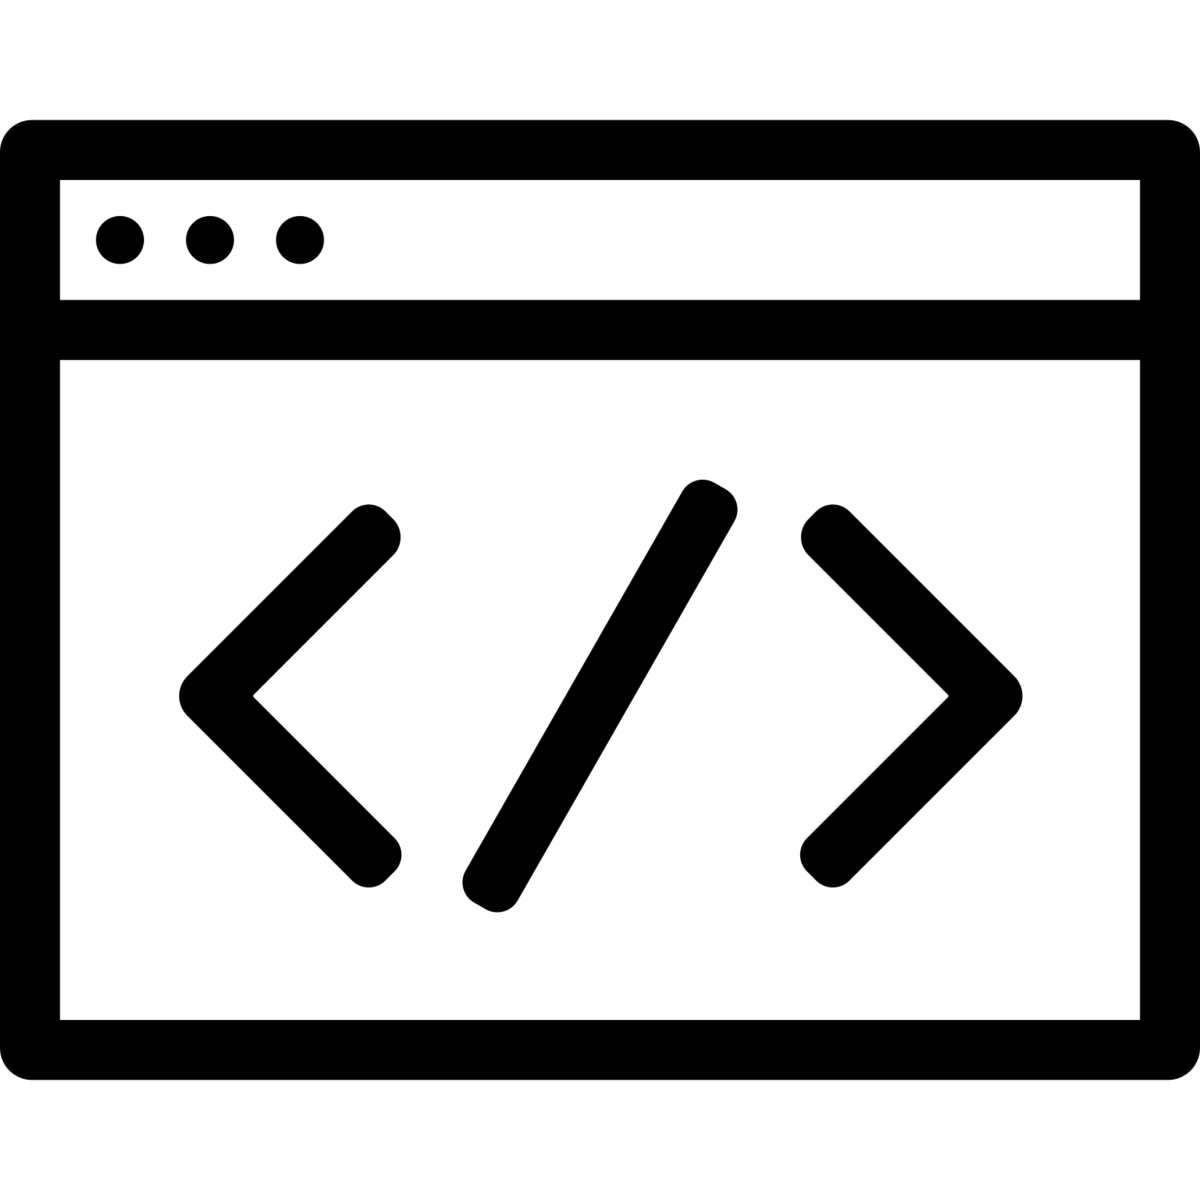
\includegraphics[width=2cm]{figures/srccode.png}};
    \node (srcLabel) [above=-0.3cm of sourceCode,visible on=<2->] {Source Code};
    \node (compiler) [right of=sourceCode, visible on=<1->] {
\includegraphics[width=1cm]{figures/c.png}};
    \node (compilerLabel) [above=-0.3cm of compiler, visible on=<1->] {C Compiler};
    \node (outputCode) [right of=compiler, visible on=<3->] {
\includegraphics[width=2.5cm]{figures/binary.png}};
    \node (outputLabel) [above=-0.55cm of outputCode, visible on=<3->] {Machine Code};


    \draw [->, thick, visible on=<2->, shorten >= 0.6cm] (sourceCode) -- (compiler);
    \draw [->, thick, visible on=<3->, shorten <= 0.6cm] (compiler) -- (outputCode);
    \node[draw,line width=2pt, rounded corners=5pt, fit=(compiler)(compilerLabel)] {};

    \node (front) [visible on=<4->, below=0.5cm of sourceCode] {\Large Front};
    \node (frontDesc) [visible on=<5->, below=0.2cm of front, xshift=1cm]
    {
      \begin{minipage}{5cm}
        \footnotesize
      \begin{itemize}
        \setlength\itemsep{-0.5em}
        \item Parsing
        \item Lexing
        \item Typechecking
      \end{itemize}
      \end{minipage}
    };
    \node (frontbug) [below=1.5cm of front,visible on=<8->] {\color{magenta} 0 GCC, 10 LLVM};
    \node (middle) [right of=front, visible on=<4->] {\Large Middle};
    \node (middleDesc) [visible on=<6->, below=0.2cm of middle, xshift=0.8cm]
    {
      \begin{minipage}{5cm}
        \footnotesize
      \begin{itemize}
        \setlength\itemsep{-0.5em}
        \item IR Optimizations
      \end{itemize}
      \end{minipage}
    };
    \node (middlebug) [below=1.5cm of middle,visible on=<9->] {\color{magenta} 49 GCC, 75 LLVM};
    \node (back) [right of=middle, visible on=<4->] {\Large Back};
    \node (dummy) [below=0.4 of middle]{};
    \node (backDesc) [visible on=<7->, below=0.2cm of back, xshift=1cm]
    {
      \begin{minipage}{5cm}
        \footnotesize
      \begin{itemize}
        \setlength\itemsep{-0.5em}
        \item Assembly Generation
        \item Register Allocation
      \end{itemize}
      \end{minipage}
    };
    \node (backbug) [below=1.5cm of back,visible on=<10->] {\color{magenta} 17 GCC, 74 LLVM};

    \node (citation) [below=2cm of middle, visible on=<8->] {Bug Finding \bf (Yang
      et al., 2011)};

    \draw [dashed, gray, visible on=<4->, shorten >= 0.3cm, shorten <= 0.7cm] (compiler) -- (front);
    \draw [dashed, gray, visible on=<4->, shorten >= 0.3cm, shorten <= 0.7cm] (compiler) -- (back);

    \draw [->, thick, visible on=<4->, shorten >= 0.3cm, shorten <= 0.3cm] (front) -- (middle);
    \draw [->, thick, visible on=<4->, shorten <= 0.3cm, shorten >= 0.3cm] (middle) -- (back);
    \node[draw,line width=2pt, visible on=<4->, rounded corners=2pt, fit=(front)] {};
    \node[draw,line width=2pt, visible on=<4->, rounded corners=2pt, fit=(middle)] {};
    \node[draw,line width=2pt, visible on=<4->, rounded corners=2pt, fit=(back)] {};
    % \node[draw,line width=2pt, visible on=<8->, rounded corners=2pt, color=red,
      % fit=(middle)(back)(dummy), inner xsep =0.4cm, inner ysep =0.5cm,
      % label={[name=l, visible on=<8->] \color{red} Verified}] {};
  \end{tikzpicture}

  \vspace{-1cm}

  \begin{tikzpicture}[node distance=3.5cm]
  \end{tikzpicture}
  \end{center}
\end{frame}

\begin{frame}{Verified Compilers}
  \begin{center}
  {\Large Avoid bugs through verification!}

  \onslide<2->{
  \begin{tikzpicture}
  \node (clogo) {
\includegraphics[width=2cm]{figures/c.png}};
  \node[below=0cm of clogo] (c) {CompCert \textbf{(Leroy et al., 2009)}};
    \node (compCertDesc) [below=0cm of c]
    {
      \begin{minipage}{3cm}
      \begin{itemize}
        \setlength\itemsep{-0.5em}
        \item<2-> Verified in Coq
        \item<2-> 100,000 lines
      \end{itemize}
      \end{minipage}
    };

  \node[right=4cm of clogo] (cakelogo) {
\includegraphics[width=1.5cm]{figures/cakeml.png}};
  \node[right=1.5cm of c] (cake) {CakeML \textbf{(Kumar et al., 2014)}};
    \node (cakeDesc) [below=0cm of cake]
    {
      \begin{minipage}{4cm}
      \begin{itemize}
        \setlength\itemsep{-0.5em}
        \item<2-> Verified in HOL4
      \end{itemize}
      \end{minipage}
    };

  \end{tikzpicture}}
  \end{center}
\end{frame}

\begin{frame}{CompCert: A Case Study in Verified Compilation}
  \begin{center}
  \begin{tikzpicture}[node distance=3.7cm]
    \node (sourceCode) [visible on=<1->] {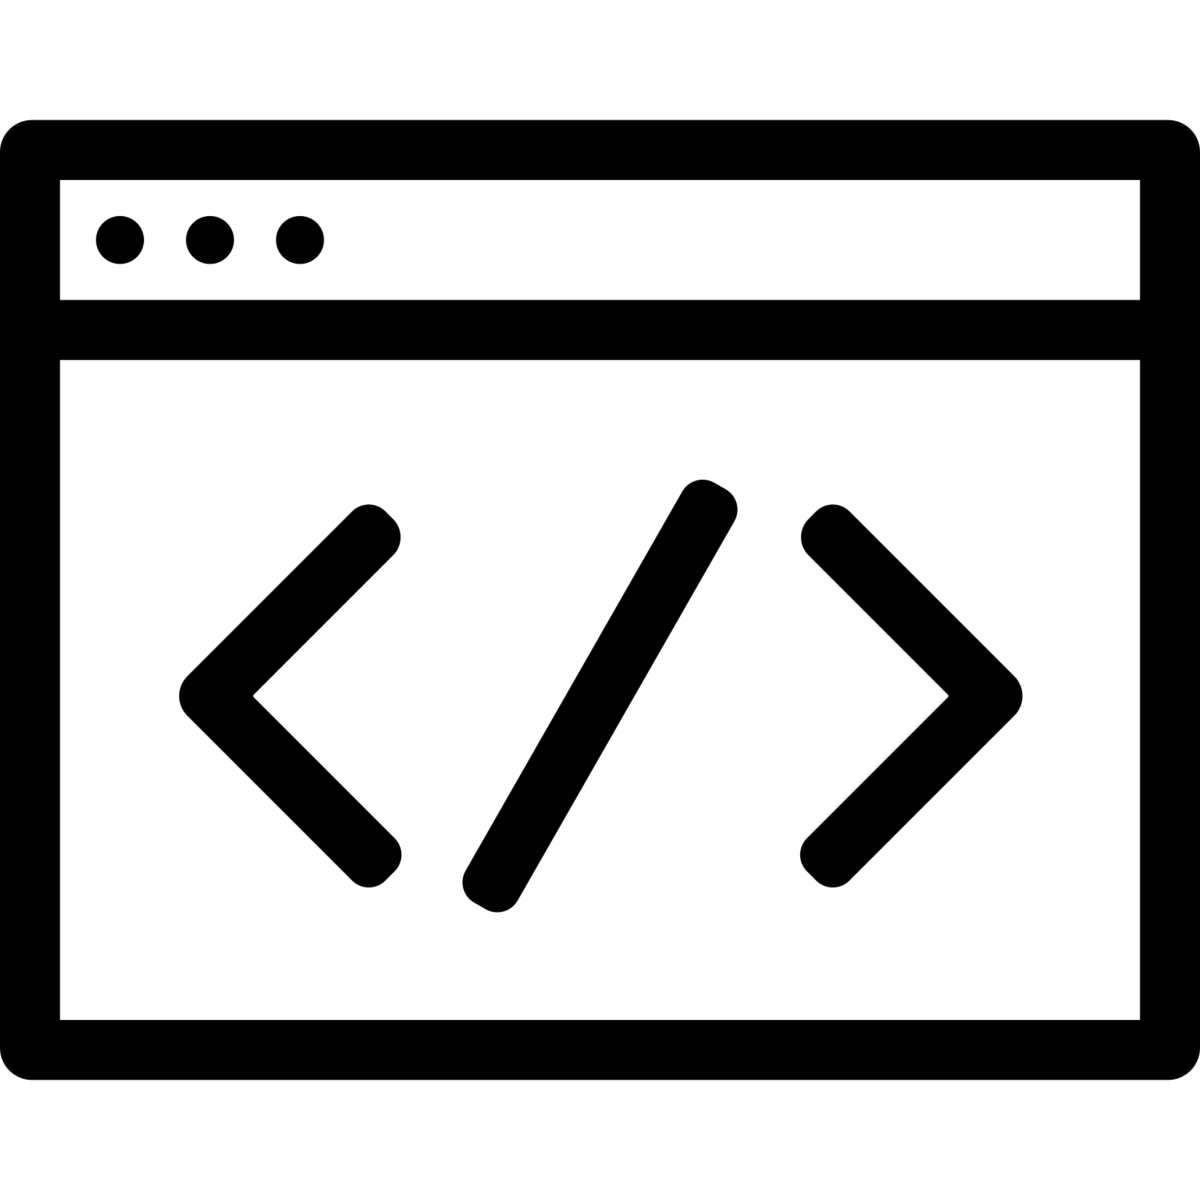
\includegraphics[width=2cm]{figures/srccode.png}};
    \node (srcLabel) [above=-0.3cm of sourceCode,visible on=<1->] {Source Code};
    \node (compiler) [right of=sourceCode, visible on=<1->] {
\includegraphics[width=1cm]{figures/c.png}};
    \node (compilerLabel) [above=-0.3cm of compiler, visible on=<1->] {CompCert};
    \node (outputCode) [right of=compiler, visible on=<1->] {
\includegraphics[width=2.5cm]{figures/binary.png}};
    \node (outputLabel) [above=-0.55cm of outputCode, visible on=<1->] {Machine Code};


    \draw [->, thick, visible on=<1->, shorten >= 0.6cm] (sourceCode) -- (compiler);
    \draw [->, thick, visible on=<1->, shorten <= 0.6cm] (compiler) -- (outputCode);
    \node[draw,line width=2pt, rounded corners=5pt, fit=(compiler)(compilerLabel)] {};

    \node (front) [visible on=<1->, below=0.5cm of sourceCode] {\Large Front};
    \node (frontbug) [below=1cm of front,visible on=<2->] {\color{magenta} 0 GCC, 10 LLVM};
    \node (frontbugc) [below=0cm of frontbug,visible on=<5->] {\color{blue} 6 CompCert???};
    \node (middle) [right of=front, visible on=<1->] {\Large Middle};
    \node (middlebug) [below=1cm of middle,visible on=<2->] {\color{magenta} 49 GCC, 75 LLVM};
    \node (middlebugc) [below=0cm of middlebug,visible on=<4->] {\color{blue} 0 CompCert};
    \node (back) [right of=middle, visible on=<1->] {\Large Back};
    \node (dummy) [below=0.4 of middle]{};
    \node (backbug) [below=1cm of back,visible on=<2->] {\color{magenta} 17 GCC, 74 LLVM};
    \node (backbugc) [below=0cm of backbug,visible on=<3->] {\color{blue} 0 CompCert};

    \node (citation) [below=2cm of middle, visible on=<2->] {\bf (Yang
      et al., 2011)};

    \draw [dashed, gray, visible on=<1->, shorten >= 0.3cm, shorten <= 0.7cm] (compiler) -- (front);
    \draw [dashed, gray, visible on=<1->, shorten >= 0.3cm, shorten <= 0.7cm] (compiler) -- (back);

    \draw [->, thick, visible on=<1->, shorten >= 0.3cm, shorten <= 0.3cm] (front) -- (middle);
    \draw [->, thick, visible on=<1->, shorten <= 0.3cm, shorten >= 0.3cm] (middle) -- (back);
    \node[draw,line width=2pt, visible on=<1->, rounded corners=2pt, fit=(front)] {};
    \node[draw,line width=2pt, visible on=<1->, rounded corners=2pt, fit=(middle)] {};
    \node[draw,line width=2pt, visible on=<1->, rounded corners=2pt, fit=(back)] {};
    \node[draw,line width=2pt, visible on=<6->, rounded corners=2pt, color=blue,
      fit=(middle)(back), inner xsep =0.5cm, inner ysep =0.5cm] (verifBox) {};
    \node[below=0.1cm, inner sep=0pt, visible on=<6->] at (verifBox.south) {\color{blue} Verified};
  \end{tikzpicture}
  \end{center}
\end{frame}

\begin{frame}{Parsing is Everywhere}
  A \emph{parser} emits structured data from an input string

  \onslide<2->{
  \begin{center}
  \begin{tikzpicture}[
    treenode/.style = {shape=rectangle, rounded corners,
    draw, align=center, font=\large,
    top color=white, bottom color=white!20},
    line/.style={draw, -latex'},
    edge from parent/.style={draw,-latex'},
    level 1/.style={sibling distance=20mm, level distance=0.5cm},
    level 2/.style={sibling distance=1cm, level distance=1cm}]

    \node (src) {\Large \texttt{"1+2*3"}};

    \node[right=2cm of src, shape=rectangle, draw] (parser) {\Large Parser};

    \node[right=3cm of parser, treenode] (tree) {$+$}
    child { node[treenode] (one) {$1$} }
    child { node[treenode] (times){$\ast$}
        child { node[treenode] {$2$} }
        child { node[treenode] {$3$} }
      };


  \draw [->, thick, shorten <= 0.3cm, shorten >= 0.3cm] (src) -- (parser);
  \draw [->, thick, shorten <= 0.3cm, shorten >= 1cm] (parser) -- (tree);

  \end{tikzpicture}
  \end{center}
  }

  \onslide<3->{
  Ubiquitous in computer science,
  \begin{itemize}
    \item<4-> Data deserialization
    \item<5-> \textbf{Programming language implementation}
      \begin{itemize}
        \item<6-> High-level source code must be understood by the machine
        \item<7-> Interpreters and compilers
      \end{itemize}
  \end{itemize}
  }
\end{frame}

\begin{frame}{Contributions of This Project}
  \begin{alertblock}{Goals}
    \begin{enumerate}
       \item<1-> Provide a unifying framework to reason about formal grammars
       \item<2-> Implement the framework in Agda
       \item<3-> Instantiate this framework to build verified parsers
    \end{enumerate}
  \end{alertblock}

  \onslide<4->{
  \begin{block}{Roadmap}
    \begin{enumerate}
      \item<4-> Give a type theory that describes formal grammars
      \item<4-> Internalize parsing algorithms as terms
      \item<4-> Express proofs of parsing algorithm correctness
    \end{enumerate}
  \end{block}
  }

  \onslide<5>{
    \begin{center}
    \textbf{Domain specific language} for building verified parsers
    \end{center}
  }
\end{frame}


\section{Formal Grammars}

\begin{frame}{Formal Grammars}
  A generative grammar is usually given as a set of production rules
  for producing parse trees
  \begin{itemize}
    \item In the style of Chomsky
  \end{itemize}
  \vspace{-0.7cm}
  \begin{center}
      \begin{gather*}
        S \to E + E \qquad E \to E * E \\
        E \to 1 \qquad E \to 2 \qquad E \to 3
      \end{gather*}
  \end{center}

  \begin{exampleblock}{Derivation of $1+2*3$}
    \begin{center}
  \begin{tikzpicture}[%opacity=0.5,
  treenode/.style = {shape=rectangle, rounded corners,
    draw, align=center,
    top color=white, bottom color=white!20},
    line/.style={draw, -latex'},
    edge from parent/.style={draw,-latex'},
    level 1/.style={sibling distance=20mm, level distance=0.7cm},
    level 2/.style={sibling distance=1cm, level distance=0.7cm}
    ]
    \node[treenode] (tree) {$S$}
    child { node[treenode] {$E$} child {node[treenode] {$1$}} }
    child { node[treenode] {$+$} }
    child { node[treenode] {$E$}
      child {node[treenode] {$E$} child {node[treenode] {$2$}}}
      child {node[treenode] {$*$}}
      child {node[treenode] {$E$} child {node[treenode] {$3$}}}
    }
      ;
\end{tikzpicture}
    \end{center}
  \end{exampleblock}
\end{frame}

\begin{frame}{Formal Languages and Equivalence}
  The \emph{formal language} for a grammar $g$ is the set of strings that match $g$

  \[
    L_{g} := \{ w \in \Sigma^{*} \mid \exists \text{ parse matching } w \text{ to } g\}
  \]

  \onslide<2->{
  \[
    L_{g} : \Sigma^{*} \to \mathbf{Bool}
  \]
  }

  \onslide<3->{\textbf{(Chomsky, 1963)} Grammars $g$ and $h$ are\dots}
  \begin{itemize}
    \item<4-> \emph{weakly equivalent} if they generate the same language, $L_{g} = L_{h}$
    \item<4-> \emph{strongly equivalent} if there is a bijection between their sets of parse trees, $g \cong h$
  \end{itemize}
\end{frame}

\begin{frame}{Grammars as Functions}
  An \emph{abstract formal grammar} $g$ is a function $g : \Sigma^{*} \to \Set$
  \begin{itemize}
    \item Strings are mapped to the \textbf{set of parse trees} matching $g$
  \end{itemize}

  \begin{minipage}[t]{.4\textwidth}
    \[
      \onslide<2->{g = {\color{blue} a} \otimes ({\color{magenta} b} \oplus {\color{orange} c})}
    \]
  \begin{tikzpicture}[%opacity=0.5,
  treenode/.style = {shape=rectangle, rounded corners,
    draw, align=center,
    top color=white, bottom color=white!20},
    line/.style={draw, -latex'},
    edge from parent/.style={draw,-latex'},
    level 1/.style={sibling distance=20mm, level distance=0.5cm},
    level 2/.style={sibling distance=1cm, level distance=1cm},
    visible on=<3->
    ]
  \node[treenode] (tree) {$\otimes$}
    child { node[treenode] (a) {${\color{blue} a}$} }
    child { node[treenode] (b){${\color{magenta} \mathsf{inl}}$}
        child { node[treenode] (c) {${\color{magenta} b}$} }
      };
      \node[draw, fit=(tree)(a)(b)(c),
      label={[name=l] $g(ab)$}, visible on=<3->] {};
    \node[below=2.5cm of tree] (mt) {};
    \node[below=2.5cm of a] (mta) {};
    \node[below=2.5cm of b] (mtb) {};
    \node[below=-0.2cm of mt, visible on=<4->] (mtset) {};
      \node[draw, fit=(mt)(mtset)(mta)(mtb),
      label={[name=l, visible on=<4->] $g(aa)$}, visible on=<4->] {};
\end{tikzpicture}
  \end{minipage}%
  \begin{minipage}[t]{.6\textwidth}
    \[
      \onslide<5->{h = {\color{blue} a^{*}} \otimes {\color{magenta} a^{*}}}
    \]
  \begin{tikzpicture}[%opacity=0.5,
  treenode/.style = {shape=rectangle, rounded corners,
    draw, align=center,
    top color=white, bottom color=white!20},
    line/.style={draw, -latex'},
    edge from parent/.style={draw,-latex'},
    level 1/.style={sibling distance=2cm, level distance=0.5cm},
    level 2/.style={sibling distance=1cm, level distance=1cm},
    visible on=<6->
    ]

   \node[treenode] (tree) {$\otimes$}
   child { node[treenode] (a) {${\color{blue} \mathsf{cons}}$}
     child {node[treenode] (b) {${\color{blue} a}$}}
     child {node[treenode] (c) {${\color{blue} \mathsf{nil}}$}
       child {node[treenode] {${\color{blue} \varepsilon}$}}
     }
   }
   child {node[treenode] {${\color{magenta} \mathsf{nil}}$}
     child {node {${\color{magenta} \varepsilon}$}}
     }
    ;
   \node[treenode, right=2.5cm of tree] (tree2) {$\otimes$}
   child {node[treenode] {${\color{blue} \mathsf{nil}}$}
     child {node {${\color{blue} \varepsilon}$}}
   }
   child { node[treenode] (x) {${\color{magenta} \mathsf{cons}}$}
     child {node[treenode] (y){${\color{magenta} a}$}}
     child {node[treenode] (z){${\color{magenta} \mathsf{nil}}$}
       child {node[treenode] (w){${\color{magenta} \varepsilon}$}}
     }
   }
    ;
      \node[draw, fit=(tree)(a)(b)(c)(x)(y)(z)(w),
      label={[name=l] $h(a)$}, visible on=<6->] {};
\end{tikzpicture}
  \end{minipage}%
\end{frame}

\begin{frame}[fragile]{Productions as Constructors}
  \begin{center}
      \begin{gather*}
        S \to E + E \qquad E \to E * E \\
        E \to 1 \qquad E \to 2 \qquad E \to 3
      \end{gather*}

  \end{center}

  Productions can be viewed like inductive data types

  \begin{center}
      \begin{lstlisting}
            data Expr =
                Sum of Exp * Exp |
                Prod of Exp * Exp |
                One |
                Two |
                Three
      \end{lstlisting}
  \end{center}
\end{frame}

\section{Grammars as Types}

\begin{frame}{Why Types?}
  \textbf{(Firsov and Uustalu, 2015)} provide a verified context-free grammar parser, up to weak equivalence

  \begin{itemize}
    \item<2-> Suggest an extension where parse trees are first-class objects
    \item<3-> Parse trees serve as proofs of language membership
    \item<4-> Under Curry-Howard, expect a corresponding type system
  \end{itemize}

  \todoin{Curry-Howard picture}

  \onslide<5->{Grammar
  $g : \Sigma^{*} \to \Set$
  can be viewed as a functor}

  \begin{itemize}
    \item<6-> $\Sigma^{*}$ viewed as a discrete category
    \item<7-> Functors into $\Set$ --- presheaves --- have significant structure
    \item<8-> Presheaves model dependent type theory
    \item<9-> Design a type theory where grammars are the intended model
  \end{itemize}
\end{frame}

% TODO examples w/o kleene star
% TODO different title
\begin{frame}{Grammars as Types}
  Types are \textbf{grammars}, and terms are
  \only<1-5>{\textbf{parse trees}}\only<6->{\textbf{parse transformers}}

  \[
    w : \Sigma^{*} \vdash p : g
  \]

  \onslide<2->{
  Think of $p$ as a \textbf{proof}
  \begin{itemize}
    \item Evidence that $w$ matches $g$
  \end{itemize}}

  \vspace{-0.5cm}
  \onslide<3->{
  \[
    x : a \otimes a \vdash \mathsf{let}~(a_{1},a_{2}) = x~\mathsf{in}~ \mathsf{cons}(a_{1}, \mathsf{cons}(a_{2}, \mathsf{nil})) : a^{*}
  \]
  }
  \vspace{-0.5cm}
  \onslide<4->{
  \[
    \alert<6>{x : a , y : b^{*}} \vdash (x , y) : a \otimes b^{*}
  \]
  }
  \vspace{-0.5cm}
  \onslide<5->{
    \[
      \Delta \vdash M : g
    \]
    $\Delta$ is an ordered list of resources that get turned into a parse $M$ of $g$
  }

\end{frame}

\begin{frame}{Separation Logic and Linear Logic Influence}
  Separation logic
  \begin{itemize}
    \item<1-> Reason about disjoint heap regions (disjoint substrings)
    \item<2-> Context extension concatenates resources
  \end{itemize}
  \onslide<2->{
  \[
    \inferrule
    {\Delta \vdash x : g \\ \Delta' \vdash y : h}
    {\Delta , \Delta' \vdash (x , y) : g \otimes h}
  \]}

  \onslide<3->{Ordered, linear logic}
  \begin{itemize}
    \item<3-> Resource-sensitive reasoning
    \item<3-> Using a linear resource consumes it, no duplication or discarding
    \item<3-> i.e.\ characters appear as written, and in order
  \end{itemize}
  \begin{align*}
    \onslide<4->{x : c, y : a, z : t & \vdash (x,y,z) : c \otimes a \otimes t} \\
    \onslide<5->{{\color{red} x : c, y : a, z : t} & {~\color{red} \not \vdash (y,x,z) : a \otimes c \otimes t}} \\
    \onslide<6->{{\color{red} x : c, y : a, z : t} & {~\color{red} \not \vdash (x,y,z,z) : c \otimes a \otimes t \otimes t}} \\
    \onslide<7->{{\color{red} x : c, y : a, z : t} & {~\color{red} \not \vdash (y,z) : a \otimes t}} \\
  \end{align*}
\end{frame}

\begin{frame}{Type Constructors}
  \begin{center}
  \begin{tabular}{c c}
    \textbf{Constructor} & \textbf{Syntax} \\
    Empty String & $\varepsilon$ \\
    Literal & $c \in \Sigma$ \\
    Concatenation & $g \otimes h$ \\
    Disjunction & $g \oplus h$ \\
    Conjunction & $g \amp h$ \\
    Top & $\top$ \\
    Bottom & $\bot$ \\
    Implication & $g \Rightarrow h$ \\
    Negation & $\neg g$ \\
    Least-fixed Point & $\mu x . g$ \\
    Linear Functions & $g \lto h$ \\
     & $g \tol h$ \\
    LNL Dependent Types & $\LinPiTy {x} {X} {g}$ \\
    & $\LinSigTy {x} {X} {g}$
  \end{tabular}
  \end{center}
\end{frame}

\begin{frame}{Non-linear Types}
  Types up until now have been \emph{linear} types

  As in \textbf{(Krishnaswami et al., 2015)}, we make use of a linear fragment and a non-linear fragment
  \begin{itemize}
    \item Synthesizes dependent types and linear types
  \end{itemize}

  \onslide<2->{
  The non-linear fragment is ordinary Martin-L\"of type theory
  \begin{itemize}
    \item Can have linear types depend on non-linear types
    \begin{gather*}
      \LinPiTy {x}{X}{g} \\
      \LinSigTy {x}{X}{g}
    \end{gather*}
    \item Used for bringing ordinary mathematical constructs into scope
    \item i.e. can define a type of non-linear stacks for PDAs
  \end{itemize}
  }
\end{frame}

\begin{frame}{Linear Function Types}
  \todoin{Brzozowski derivatives}
  \todoin{example of parsing $g \lto h$}
\end{frame}

\begin{frame}{Fixed-point Operator}
  Recursive grammars are ubiquitous in practice
  \begin{itemize}
    \item Using only $c \in \Sigma$, $\varepsilon$, $\otimes$, $\oplus$, and $\amp$ we cannot describe infinite languages
  \end{itemize}

  \onslide<3->{
    \[
      \inferrule{\Delta \vdash e : A[\mu x . A / x]}{\Delta \vdash \mathsf{cons}~e : \mu x . A}
    \]
  }
  \onslide<4->{
    \[
      g^{*} := \mu {\color{YellowOrange} x} . ({\color{blue}\varepsilon} \oplus ({\color{magenta} g} \otimes {\color{YellowOrange} x}))
    \]
  }
  \onslide<5->{
    \[
      g^{*} \cong {\color{blue} \varepsilon} \oplus ({\color{magenta} g} \otimes {\color{YellowOrange} g^{*}})
    \]
  }
  \onslide<6->{
    Inductive data type with constructors,
    \begin{itemize}
      \item<6-> ${\color{blue} \bullet} \vdash \mathsf{nil} : g^{*}$
      \item<6->
            ${\color{magenta} x : g}, {\color{YellowOrange} y : g^{*}} \vdash \mathsf{cons}(x , y) : g^{*}$
    \end{itemize}
  }
\end{frame}

% \begin{frame}{Kleene Star Elimination}
%   Constructors
%   \[
%     {\color{blue} \bullet \vdash \mathsf{nil} : g^{*}} \qquad {\color{magenta} x : g, y : g^{*} \vdash \mathsf{cons}(x , y) : g^{*}}
%   \]
%   \onslide<2->{
%   Eliminator
%   \[
%       \inferrule*[Right=$*$Elim]
%       {
%         {\color{blue} \bullet \vdash p_{\varepsilon} : h} \\
%         {\color{magenta} x : g, y : h \vdash p_{*} : h}
%       }
%       {p : g^{*} \vdash \mathsf{fold}(p_{\varepsilon}, p_{*})(p) : h}
%     \]
%   }
%   \onslide<3->{
%     \begin{exampleblock}{Example}
%       \[
%       \inferrule
%       {
%         \onslide<4->{        \bullet \vdash \mathsf{nil : a^{*}}} \\
%         \onslide<5->{x : aa, y : (a)^{*} \vdash p_{*} : a^{*}}
%       }
%       {p : (aa)^{*} \vdash \mathsf{fold}(\mathsf{nil},p_{*})(p) : a^{*}}
%       \]
%     \end{exampleblock}
%   }
% \end{frame}

\begin{frame}{Notions of Equivalence}
  Logical equivalence from functional programming
  \begin{gather*}
    x : A \vdash p(x) : B \\
    y : B \vdash q(y) : A
  \end{gather*}

  Captures Chomsky's weak equivalence

  \onslide<2->{
  Induced notion of isomorphism in our type system
  \begin{gather*}
    p(q(y)) = y \\
    q(p(x)) = x
  \end{gather*}
  is Chomsky's strong equivalence
  \todoin{Polish this slide}
  }
\end{frame}

\begin{frame}{Implementation}
  Implement the type theory by shallowly embedding it in Agda
  \begin{itemize}
    \item Leverage Agda's type system as a host for our logic
    \item Parsers written in our syntax are \textbf{intrinsically verified}
       \begin{itemize}
          \item Type system carries proofs of correctness
       \end{itemize}
  \end{itemize}
  \begin{center}
  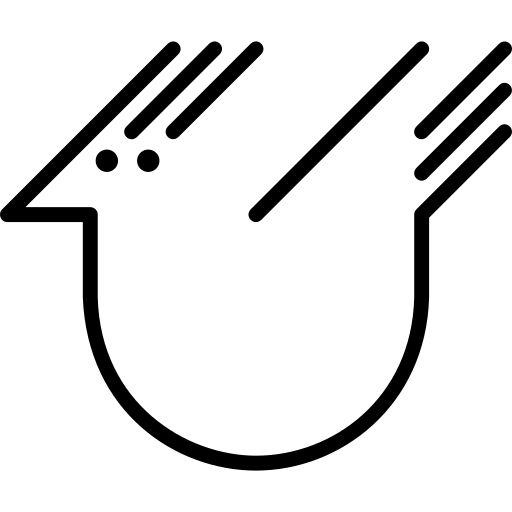
\includegraphics[width=3cm]{figures/agda.png}
  \end{center}
\end{frame}

\section{Building a Parser}

\begin{frame}{A Sample Parsing Algorithm}
  \begin{alertblock}{Benchmark Parser}
  Build a verified regular expression parser
  \end{alertblock}
  \begin{block}{Sample Algorithm}
    \begin{enumerate}
      \item Prove that regular expressions are equivalent to NFAs \textbf{(Formalized)}
      \item Prove that NFAs are equivalent to DFAs \textbf{(WIP)}
      \item Build a parser term for DFA grammars \textbf{(Formalized)}
    \end{enumerate}
  \end{block}
\end{frame}

\begin{frame}{A Specification for Parsers}
  \onslide<1->{\alert<1>{Input string $w$}} \qquad \onslide<2->{\alert<2>{Grammar $g$}}

  \onslide<3->{
  \begin{block}{\alert<3>{Parser Term}}
    $$ \alert<4>{w : \Sigma^{*}} \vdash \alert<7>{\mathsf{parse}_{g}(w)} : \alert<5>{g} \oplus \alert<6>{\neg g} $$
  \end{block}}

  \onslide<8->{
  \begin{exampleblock}{Example}
    \begin{minipage}{.7\textwidth}
    \onslide<8->{\alert<8>{$g = a \otimes (b \oplus c)$}}

    \onslide<9->{\alert<9>{$w = ab$}}
    \onslide<10->{$\longrightarrow \mathsf{parse}_{g}(w) = {\color{blue} \mathsf{inl}(p_{g})} : \alert<10>{g} \oplus \neg g$
    \quad {\LARGE \color{blue} \cmark}}

    \onslide<11->{\alert<11>{$w = ad$}}
    \onslide<12->{$\longrightarrow \mathsf{parse}_{g}(w) = {\color{magenta} \mathsf{inr}(p_{\neg g})} : g \oplus \alert<12>{\neg g}$
    \quad {\LARGE \color{magenta} \xmark}}
    \end{minipage}%
    \begin{minipage}{.3\textwidth}
      \begin{center}
        \begin{tikzpicture}[%opacity=0.5,
        treenode/.style = {shape=rectangle, rounded corners,
          draw, align=center,
          top color=white, bottom color=white!20},
          line/.style={draw, -latex'},
          edge from parent/.style={draw,-latex'},
          level 1/.style={sibling distance=20mm, level distance=1cm},
          level 2/.style={sibling distance=1cm, level distance=1cm},
          scale = 0.7, visible on=<10->
          ]
        \node[treenode] (tree) {$\otimes$}
          child {node[treenode] {$a$}}
          child {node[treenode] {$\mathsf{inl}$}
            child {node[treenode] {$b$}}}
          ;

        \node[above=0.1cm of tree, visible on=<10->] {$\color{blue} p_{g}$};
        \end{tikzpicture}
      \end{center}
    \end{minipage}%
  \end{exampleblock}}
\end{frame}

\begin{frame}{Grammars and Their Automata}
  Characterize classes of grammars based on structure of their productions

  \begin{block}{Chomsky Hierarchy}
  \begin{center}
    \begin{tabular}{c c}
      \textbf{Grammar Class} & \textbf{Automata} \\
      Regular & Finite \\
      Context-free & Pushdown \\
      Context-sensitive & Linear-bounded \\
      Unrestricted & Turing machine
    \end{tabular}
  \end{center}
  \end{block}

  \begin{itemize}
    \item Correspondence between classes of grammars and the classes of machines that recognize them
    \item Can encode the entire hierarchy in our syntax
    \item Describe automata as grammars in the type system
  \end{itemize}
\end{frame}

\begin{frame}{A Nondeterministic Finite Automaton} $g = a^{*} \otimes (b \oplus c)$

  \only<1-21>{\alert<21>{$\alert<7>{w} = \alert<8-10>{a} \alert<11-13>{a} \alert<14-16>{b}
    \only<18-19>{\otimes \alert{\varepsilon}}$} \quad \only<21>{ {\Large \color{blue} \cmark}}}

  \onslide<3->{
  \begin{center}
  \begin{tikzpicture}[node distance = 25mm ]
    \Large
    \alert<4,8>{\node (0) {start};}
    \alert<4,8,10-11,13-14>{\node[state, right of=0] (1) {$q_{1}$};}
    \alert<5,20>{\node[state, right of=1, accepting] (2) {$q_{2}$};}
    \alert<16-17>{\node[state, below of=1] (3) {$q_{3}$};}

    \alert<15>{\draw[->] (1) edge[left] node{$b$} (3);}
    \draw[->] (1) edge[above] node{$c$} (2);
    \alert<9,12>{\draw[->] (1) edge[loop above] node{$a$} (1);}
    \alert<19>{\draw[->] (3) edge[below] node{$\varepsilon$} (2);}
    \alert<4,8>{\draw[->] (0) edge[above] node{} (1);}
  \end{tikzpicture}
  \end{center}}
\end{frame}

\begin{frame}{Automata as Grammars}
  $g = a^{*} \otimes (b \oplus c)$

  \onslide<2-21>{\alert<21>{$\alert<7>{w} = \alert<8-10>{a} \otimes  \alert<11-13>{a} \otimes \alert<14-16>{b}
    \only<18-19>{\otimes \alert{\varepsilon}}$} \quad \only<21>{ {\Large \color{blue} \cmark}}}

  \begin{center}
  \begin{minipage}{.5\textwidth}
  \onslide<3->{
  \begin{tikzpicture}[node distance = 15mm, scale=0.4]
    \alert<4,8>{\node (0) {start};}
    \alert<4,8,10-11,13-14>{\node[state, right of=0] (1) {$q_{1}$};}
    \alert<5,20>{\node[state, right of=1, accepting] (2) {$q_{2}$};}
    \alert<16-17>{\node[state, below of=1] (3) {$q_{3}$};}

    \alert<15>{\draw[->] (1) edge[left] node{$b$} (3);}
    \draw[->] (1) edge[above] node{$c$} (2);
    \alert<9,12>{\draw[->] (1) edge[loop above] node{$a$} (1);}
    \alert<19>{\draw[->] (3) edge[below] node{$\varepsilon$} (2);}
    \alert<4,8>{\draw[->] (0) edge[above] node{} (1);}
  \end{tikzpicture}
  }
  \end{minipage}%
  \begin{minipage}{.5\textwidth}
    \onslide<4->{
    Define a type of traces between two states

    \onslide<4->{$$ \mathsf{Trace}(q_{1}, q_{2}) =$$
    \begin{equation*}
      \mu
      \begin{pmatrix}
        \alert<8,10,11,13,14>{g_{q_{1}}} := & \alert<9,12>{(a \otimes g_{q_{1}})} \\ & \oplus  ( c \otimes g_{q_{2}} ) \\ & \oplus \alert<15>{(b \otimes g_{q_{3}})} \\
        \alert<20>{g_{q_{2}}} := & \alert<5,20>{\varepsilon} \\
        \alert<16,17>{g_{q_{3}}} := & \alert<19>{g_{q_{2}}} \\
      \end{pmatrix}. \alert<4>{\color<21>{blue} g_{q_{1}}}
    \end{equation*}}
    }
  \end{minipage}
  \end{center}
\end{frame}

% \begin{frame}{Determinism}
%   A \emph{deterministic} finite automaton (DFA) has no $\varepsilon$-transitions and for every state there is exactly one outgoing transition for each $c \in \Sigma$.

%    \begin{center}
%    \begin{tikzpicture}[node distance = 15mm, scale=0.4]
%         \node (0) {start};
%         \node[state, right of=0] (1) {$q_{1}$};
%         \node[state, right of=1, accepting] (2) {$q_{2}$};
%         \node[state, below of=1] (3) {$q_{3}$};

%         \draw[->] (1) edge[left] node{$b$} (3);
%         \draw[->] (1) edge[above,bend left] node{$c$} (2);
%         \draw[->] (2) edge[above,bend left] node{$b$} (1);
%         \draw[->] (2) edge[right, bend left] node{$a,c$} (3);
%         \draw[->] (1) edge[loop above] node{$a$} (1);
%         \draw[->] (3) edge[loop below] node{$a,b,c$} (3);
%         \draw[->] (0) edge[above] node{} (1);
%       \end{tikzpicture}
%     \end{center}

%     Determinism implies unambiguity --- only one trace per input string
% \end{frame}

% \begin{frame}{Defining a Parser Term for Deterministic Automata}
%   $D$ a DFA grammar

%   \[ w : \only<1>{\Sigma^{*}}\only<2->{\left( \bigoplus_{c \in \Sigma} c \right)^{*}} \vdash \mathsf{parse}_{D}(w) : \mathsf{AccTrace}_{D} \oplus \top \]

%   \onslide<3->{Define with Kleene star eliminator!}

%   \onslide<4->{
%     \[
%       A := \overline{\sum_{q : Q}} \mathsf{Trace}_{D}(q_{init}, q)
%     \]
%   \onslide<5->{
%   \[
%     \inferrule*[Right=$*$Elim]
%     {
%       \onslide<6->{\bullet \vdash p_{\varepsilon} : A} \\
%       \onslide<7->{x : A, y : \left( \bigoplus_{c : \Sigma} c \right) \vdash p_{*} : A}
%     }
%     {w : \left( \bigoplus_{c \in \Sigma} c \right)^{*} \vdash M : A}
%   \]}
%   }
%   \todoin{Graphics defining a parser for DFAs}
% \end{frame}

\section{Next Steps and Future Work}

\begin{frame}{More Expressive Grammar Classes}
  \begin{itemize}
    \item<1-> Conclude the regular expression benchmark
    \item<2-> Extend to (deterministic) context free grammar parsing algorithms
        \begin{itemize}
          \item<3-> Emit a verified parser generator for CFGs
        \end{itemize}
    \item<4-> Restricted forms of context sensitivity
        \begin{itemize}
          \item<5-> Such as the interval parsing grammars in \textbf{(Zhang et al., 2023)}
        \end{itemize}
  \end{itemize}
\end{frame}

\begin{frame}{Related Work}
  \onslide<1->{Grammar Formalisms}
  \begin{itemize}
    \item Kleene Algebra --- algebraic reasoning about regular expressions
    \item<2-> \textbf{(Krishnaswami and Yallop, 2019)} develop LL(1) parsers for context-free expressions using typing
  \end{itemize}

  \onslide<3->{Verified Parsers}
  \begin{itemize}
    \item<3-> CompCert team rewrites parser and gives a validation procedure for LR(1) parsers \textbf{(Jourdan et al, 2012)}
    \item<4-> CoStar \textbf{(Lasser et al., 2023)} gives a verified predictive
          parser for non-left-recursive context free grammars (CFGs)
    \item<5-> \textbf{(Danielsson, 2010)} gives a verified parser combinator library
          in Agda for non-left recursive CFGs
    \item<6-> \textbf{(Firsov and Uustalu, 2015)} give a verified parser for arbitrary CFGs, up to weak equivalence
  \end{itemize}
\end{frame}

\begin{frame}{Generalizations}
  Semantics actions
  \begin{itemize}
    \item Perform semantic analysis of code during parsing
    \item i.e.\ evaluate arithmetic expressions while parsing
  \end{itemize}

  \onslide<2->{
    In this talk, we made a syntax to reason about parsing as a function $\Sigma^{*} \to \Set$

    We can instead map from tree structured data instead of $\Sigma^{*}$
    \begin{itemize}
      \item Type theory for reasoning about typechecking algorithm correctness
      \item Stranger type theory
    \end{itemize}
  }
\end{frame}

\begin{frame}[standout]
  Questions?
\end{frame}

% \begin{frame}{(Lack of) Structural Rules}
%   Omit these structural rules that usually appear in intuitionistic logic

%   \begin{mathpar}
%     \onslide<2->{
%     \only<2>{\inferrule*[Right=Weak]{\Delta \vdash M : g}{\Delta , x : A \vdash M : g}}
%     \only<3->{\xcancel{\inferrule*[Right=Weak]{\Delta \vdash M : g}{\Delta , x : A \vdash M : g}}}}

%     \and

%     \onslide<4->{

%     \only<4>{\inferrule*[Right=Contr]{\Delta , x : A , y : A \vdash  M : g}{\Delta , z : A \vdash
%       M[ z / x , z / y ] : g}}
%     \only<5->{\xcancel{\inferrule*[Right=Contr]{\Delta , x : A , y : A \vdash  M : g}{\Delta , z : A \vdash
%       M[ z / x , z / y ] : g}}}
%      }

%     \\

%     \onslide<6->{
%     \only<6>{\inferrule*[Right=Exch]{\Delta , \Delta' \vdash M : g}{\Delta' , \Delta
%       \vdash M : g}}
%     \only<7->{\xcancel{\inferrule*[Right=Exch]{\Delta , \Delta' \vdash M : g}{\Delta' , \Delta
%       \vdash M : g}}}}
%   \end{mathpar}

%   \onslide<8->{Entire context must be used, \emph{exactly once} and in order}

%   \onslide<9->{Just like when reading a word}
% \end{frame}

% \begin{frame}{Backup slides for connectives}
%   Have examples for each connective
% \end{frame}

\end{document}
